\documentclass[12pt]{article}

\usepackage{graphicx}
\usepackage{titling}
\usepackage{amsmath}
\usepackage{amssymb}
% \usepackage{tensor}
% \usepackage{ragged2e}
\usepackage{lastpage}
\usepackage[margin=2.5cm]{geometry}
\usepackage{blindtext}
\usepackage{titlesec}
\usepackage{amssymb}
\usepackage[colorlinks=true, linkcolor=blue]{hyperref}
% \usepackage{changepage}
\begin{document}


\begin{center}
    {\LARGE Stochastic Barrel Pyrolysis \\ [0.5cm]
    \large Joe Salter}
\end{center}


\section{Introduction}
We consider PuO and another material which is combustible. Considerations at the start will be general, but we will ultimately impose a slab geometry. The equations to be coupled are the sourced heat conduction equation and the time-dependent neutron diffusion equation with delayed precursors.

\subsection{Heat Conduction}
The sourced conduction equation takes the form 
\begin{equation}
    \rho (\mathbf{r}) C_p (\mathbf{r}) \frac{\partial T(\bold{r},t)}{\partial t}=\bold{\nabla} \cdot (K(\mathbf{r})\bold{\nabla} T) + S(\bold{r},t). \label{SCE}
\end{equation}
We split the source into two parts, 
\begin{equation}
    S(\bold{r},t)=S_{fission}+S_{combustion}.
\end{equation}
$S_{combustion}$ arises from decomposition, and is given by 
\begin{equation}
    S_{combustion}(\bold{r},t)=q(\mathbf{r})\left( -\frac{\partial \omega(\bold{r},t)}{\partial t} \right)
\end{equation}
with 
\begin{equation}
    -\frac{\partial \omega(\bold{r},t)}{\partial t}=k(\mathbf{r})\omega (\mathbf{r},t) exp\left(-\frac{E_{act} (\mathbf{r})}{R_g T(\mathbf{r},t)} \right).
\end{equation}
The fission source term has units of $Jm^{-3}s^{-1}$, so takes the form $E_f \times n \times v \times \Sigma_f$. Hence 
\begin{equation}
    S_{fission}=E_f \int_0 ^\infty \Sigma_f(E)\phi(\mathbf{r}, E, t)dE.
\end{equation}

\subsection{Neutron diffusion}
The time dependent NDE takes the form 
\begin{align}
    \frac{1}{v(E)} \frac{\partial \phi (\bold{r},E,t)}{\partial t}&=\bold{\nabla} \cdot (D(\bold{r}, E)\bold{\nabla} \phi)-\Sigma_a (\bold{r},E)\phi+\int_{0}^{\infty}\Sigma_s(\bold{r}, E'\rightarrow E)\phi(\bold{r},E',t)dE' \notag \\ & +\chi_p(E) \int_0 ^{\infty} \nu(E') (1-\beta)\Sigma_f (\bold{r},E')\phi(\bold{r},E',t)dE' +\sum_{i=1}^{I} \chi_{d,i}(E)\lambda_i C_i(\bold{r},t) \label{TDNDE}
\end{align}
with the precursor equations 
\begin{equation}
    \frac{\partial C_i({\bold{r},t)}}{\partial t}=\beta_i \int_0^\infty \nu(E) \Sigma_f (\bold{r},E) \phi(\bold{r}, E,t)dE-\lambda_i C_i .
\end{equation}

% \section{Solving}
% When solving the coupled thermal and neutronic equations, we should for each timestep first solve the thermal equations, then update the necessary cross sections and coefficients, and solve the neutronic equation. For this reason, a dependence on $t$ may in some cases be seen as a dependence on $T$.

\section{A Stochastic Ansatz}
\subsection{The Formalism}
Let us now introduce the machinery to deal with randomly dispersed mixtures. We define the random function $F(r,\vartheta)$ as 
\begin{equation}
    F(r,\vartheta)=1 \hspace{0.25cm}\text{If $r$ is in phase 1,} \hspace{0.25cm} F(r, \vartheta)=0 \hspace{0.25cm} \text{If $r$ is in phase 2}
\end{equation}
where $\vartheta$ is a set of realizations. We can write a random function as 
\begin{equation}
    \Psi(r, \vartheta)=\Psi_1 F+ \Psi_2 (1-F).
\end{equation}
We identify the statistical average of $F$ as the volume fraction of phase 1, and vice versa for $1-F$ :
\begin{align}
    \left< F \right>&=v \\
    \left< 1-F \right>& = 1-v.
\end{align}
We note the following properties of the random function: 

Now we apply the machinery to our system of equations. We declare phase 1 PuO and phase 2 the homogeneously averaged combustible mix. We declare all functions of $\mathbf{r}$ as random functions. 

\subsection{Stochastic Heat Conduction}
Equation \ref{SCE} becomes
\begin{align}
    \rho_1 C_{p1} \frac{\partial T_1}{\partial t}F +\rho_2 C_{p2} \frac{\partial T_2}{\partial t}(1-F)=&-F \mathbf{\nabla} \cdot \mathbf{J}_1 - \mathbf{J}_1 \cdot \mathbf{\nabla}F -(1-F) \mathbf{\nabla} \cdot \mathbf{J}_2 +\mathbf{J}_2 \cdot \mathbf{\nabla}F \notag \\ &+S_1 F + S_2 (1-F)
\end{align}
where we have introduced $\mathbf{J}(\mathbf{r})=-K(\mathbf{r})\mathbf{\nabla}T(\mathbf{r},t)$. Multiplying by $F$ and $1-F$ we get, respectively 
\begin{align}
    \rho_1 C_{p1}\frac{\partial T_1}{\partial t}F&=-F\nabla \cdot \mathbf{J}_1-\mathbf{J}_1 \cdot F\nabla F+\mathbf{J}_2 \cdot F\nabla F + S_1 F \\
    \rho_2 C_{p2}\frac{\partial T_2}{\partial t}(1-F)&=-\mathbf{J}_1 \cdot (1-F)\nabla F-(1-F)\nabla \cdot \mathbf{J}_2+\mathbf{J}_2 \cdot (1-F)\nabla F + S_2 (1-F).
\end{align}
To deal with the above, we perform a statistical average. Clearly we must take care to deal with $\left< F\nabla F \right>$. From first principles 
\begin{align}
    \left< F(x) F'(x)\right>&=\lim _{h\rightarrow 0}\left< F(x) \frac{1}{h} \left(F(x)-F(x-h)\right)\right> \notag \\
    &=\lim_{h\rightarrow 0} \frac{1}{h}\left( \left< F(x)\right>-\left< F(x)F(x-h)\right> \right).
\end{align}
To deal with $F(x)F(x-h)$, we introduce the \textbf{correlation function}, defined as 
\begin{equation}
    R(h)=\frac{\left< F(x)F(x-h)\right>-\left< F(x)\right>^2}{\left< F(x)^2\right>-\left< F(x)\right>^2}=\frac{\left< F(x)F(x-h)\right>-v^2}{v-v^2}.
\end{equation}
Hence 
\begin{align}
    \left< F(x)F'(x)\right>&=\lim_{h\rightarrow 0} \frac{1}{h}\left(v-v(1-v)R(h)-v^2\right) \notag \\
    &=\lim_{h\rightarrow 0} \frac{1}{h} \left( v-v^2-v(1-v)\left(R(0)+hR'(0)+o(h^2)\right)\right) \notag \\ 
    &=-R'(0)v(1-v) +\lim_{h\rightarrow 0}\left( v-v^2-R(0)v +R(0)v^2\right).
\end{align}
Evidently we must impose $R(0)=1$, so the limit converges, and thus we have 
\begin{equation}
    \left< F(x)F'(x)\right>=-R'(0)v(1-v).
\end{equation}
This generalises trivially to give 
\begin{equation}
    \left< F(\mathbf{r})\nabla F(\mathbf{r})\right>=-v(1-v) \nabla R(\mathbf{r}) \Bigr|_{\mathbf{r=0}}. \label{ff'}
\end{equation}
The other problem of note is the source term. $S_{fission}$ is trivial, but 
\begin{equation}
S_{combustion}=q(\mathbf{r})k(\mathbf{r})\omega(\mathbf{r},t)\exp{\left(-\frac{E_{act}(\mathbf{r})}{R_g T(\mathbf{r},t)}\right)}
\end{equation}
poses a challenge. After multiplying by $F$ and $1-F$, and statistical averaging,
\begin{align}
    vS_{combustion,1}&=q_1 k_1 \omega_1 \left<F \exp{\left(-\frac{E_{act}(\mathbf{r})}{R_g T(\mathbf{r},t)}\right)}\right> \notag \\
    (1-v)S_{combustion,2}&=q_2 k_2 \omega_2 \left<(1-F) \exp{\left(-\frac{E_{act}(\mathbf{r})}{R_g T(\mathbf{r},t)}\right)}\right>.
      \end{align}
To deal with this, we must first get the exponent in a more tractable form. We have 
\begin{align}
    \frac{E_{act}(\mathbf{r})}{T(\mathbf{r},t)}&=\frac{E_{a1}F+E_{a2}(1-F)}{T_1F+T_2(1-F)} = \frac{E_{a2}+\Delta E_a F}{T_2+\Delta TF} \notag \\
    &=\frac{E_{a2}}{T_2+\Delta TF}+\frac{\Delta E_a}{\Delta T} \frac{F}{\frac{T_2}{\Delta T}+F} \notag \\
    &=\frac{E_{a2}}{T_2+\Delta TF} + \frac{\Delta E_a}{\Delta T}- \frac{T_2}{\Delta T} \frac{\Delta E_a}{\Delta T} \frac{1}{\frac{T_2}{\Delta T}+F} \notag \\
    &=\frac{\Delta E_a}{\Delta T}+\left( E_{a2}-\frac{\Delta E_a}{\Delta T}T_2\right) \frac{1}{T_2 + \Delta T F} \notag \\
    &=\frac{\Delta E_a}{\Delta T}+\left( E_{a2}-\frac{\Delta E_a}{\Delta T}T_2\right) \int _0 ^\infty du e^{-u(T_2+\Delta TF)}.
\end{align}
We note that $E_a/R_g=T_a$. Now, exponentiating: 
\begin{align}
    \exp \left(- \frac{T_a}{T}\right)=e^{-\frac{\Delta T_a}{\Delta T}}\exp{\left[ -\left(T_{a2}-\frac{\Delta T_a}{\Delta T}T_2 \right)\int_0 ^{\infty}due^{-u(T_2+\Delta TF)} \right]}
\end{align}
And expanding in a power series: 
\begin{align}
     \exp \left( -\frac{T_a}{T}\right)&=e^{-\frac{\Delta T_a}{\Delta T}} \sum_{n=0}^\infty \frac{(-1)^n}{n!}  \left(T_{a2}-\frac{\Delta T_a}{\Delta T}T_2 \right)^n \left( \int_0 ^{\infty}due^{-u(T_2+\Delta TF)}\right)^n \notag \\
     &=e^{-\frac{\Delta T_a}{\Delta T}} \sum_{n=0}^\infty \frac{(-1)^n}{n!}  \left(T_{a2}-\frac{\Delta T_a}{\Delta T}T_2 \right)^n \left[ \int_0 ^{\infty}due^{-uT_2}\left(1+\sum_{m=1}^\infty \frac{(-1)^m}{m!}(u\Delta T)^m F^m\right)\right]^n \notag \\
     &=e^{-\frac{\Delta T_a}{\Delta T}} \sum_{n=0}^\infty \frac{(-1)^n}{n!}  \left(T_{a2}-\frac{\Delta T_a}{\Delta T}T_2 \right)^n \left[ \int_0 ^{\infty}due^{-uT_2}\left(1+F\sum_{m=1}^\infty \frac{(-1)^m}{m!}(u\Delta T)^m \right)\right]^n
\end{align}
In the above we used the slightly modified $e^{F}=1+\sum_{m=1}^\infty \frac{F^m}{m!}$. Making use of $F^n=F$ and $(1-F)^n=1-F$
\begin{align}
    F\exp{\left( -\frac{T_a}{T}\right)}&=e^{-\frac{\Delta T_a}{\Delta T}} \sum_{n=0}^\infty \frac{(-1)^n}{n!}  \left(T_{a2}-\frac{\Delta T_a}{\Delta T}T_2 \right)^n \left[ \int_0 ^{\infty}due^{-uT_2}\left(F+F\sum_{m=1}^\infty \frac{(-1)^m}{m!}(u\Delta T)^m \right)\right]^n \notag \\
    &=Fe^{-\frac{\Delta T_a}{\Delta T}} \sum_{n=0}^\infty \frac{(-1)^n}{n!}  \left(T_{a2}-\frac{\Delta T_a}{\Delta T}T_2 \right)^n \left[ \int_0 ^{\infty}due^{-uT_2}\left(1+\sum_{m=1}^\infty \frac{(-1)^m}{m!}(u\Delta T)^m \right)\right]^n \notag \\
    &=Fe^{-\frac{\Delta T_a}{\Delta T}}\exp{\left[ -\left( T_{a2}-\frac{\Delta T_a}{\Delta T}T_2\right) \int_0 ^\infty du e^{ -u(T_2+\Delta T)} \right]} \notag \\
    &=Fe^{-\frac{\Delta T_a}{\Delta T}}\exp{\left[ -\left( T_{a2}-\frac{\Delta T_a}{\Delta T}T_2\right) \frac{1}{T_2 + \Delta T} \right]}=Fe^{-\frac{T_{a1}}{T_1}}
\end{align}
and similarly 
\begin{equation}
    (1-F)\exp{\left( -\frac{T_a}{T}\right)}=(1-F)e^{-\frac{T_{a2}}{T_2}}.
\end{equation}
Hence we have 
\begin{align}
    vS_{combustion,1}&=q_1 k_1 \omega_1ve^{-\frac{T_{a1}}{T_1}}  \\
    (1-v)S_{combustion,2}&=q_2 k_2 \omega_2(1-v)e^{-\frac{T_{a2}}{T_2}}.
\end{align}
So our stochastic pyrolysis equations amount to 
\begin{align}
    \rho_1 C_{p1} \frac{\partial T_1}{\partial t}&= -\nabla \cdot \mathbf{J}_1 +(1-v)(\mathbf{J}_1-\mathbf{J}_2)\cdot \nabla R(\mathbf{r}) |_{\mathbf{r}=\mathbf{0}} + E_f \int_0 ^ \infty dE \Sigma_f \phi_1 - q_1 \frac{\partial \omega_1}{\partial t} \\
    \rho_2 C_{p2} \frac{\partial T_2}{\partial t}&= -\nabla \cdot \mathbf{J}_2 -v(\mathbf{J}_1-\mathbf{J}_2)\cdot \nabla R(\mathbf{r}) |_{\mathbf{r}=\mathbf{0}} + E_f \int_0 ^ \infty dE \Sigma_f \phi_2 - q_2 \frac{\partial \omega_2}{\partial t}
\end{align}
with the currents given by 
\begin{align}
    \mathbf{J}_1 &= -K_1 \nabla T_1 +K_1 (1-v)(T_1 -T_2) \nabla R(\mathbf{r})|_{\mathbf{r}=\mathbf{0}} \\
    \mathbf{J}_2 &= -K_2 \nabla T_2 -K_2 v(T_1 -T_2) \nabla R(\mathbf{r})|_{\mathbf{r}=\mathbf{0}}.
\end{align}
and rate of change of the volatiles 
\begin{align}
    \frac{\partial \omega _1}{\partial t} &= k_1 \omega_1 e^{-\frac{E_{a1}}{R_g T_1}} \\
    \frac{\partial \omega_2}{\partial t} &= k_2 \omega_2 e^{-\frac{E_{a2}}{R_g T_2}}.
\end{align}

\subsection{Stochastic Neutron Diffusion}
There are no new concerns in the NDE that have not been dealt with in the previous section. The stochastic NDE takes the form
\begin{align}
    \frac{1}{\upsilon(E)} \frac{\partial \phi_1 (\bold{r},E,t)}{\partial t}&= -\nabla \cdot \mathbf{Q}_1+(1-v)(\mathbf{Q}_1-\mathbf{Q}_2)\cdot \nabla R(\mathbf{r})|_{\mathbf{r}=\mathbf{0}}-\Sigma_{a1} (\bold{r},E)\phi_1 \notag \\ &+\int_{0}^{\infty}\Sigma_{s1}(\bold{r}, E'\rightarrow E)\phi_1(\bold{r},E',t)dE'  +\chi_p(E) \int_0 ^{\infty} \nu(E') (1-\beta)\Sigma_{f1} (\bold{r},E')\phi_1(\bold{r},E',t)dE' \notag \\ 
    &+\sum_{i=1}^{I} \chi_{d,i}(E)\lambda_i C_{i1}(\bold{r},t) 
    \\ \notag \\ 
    \frac{1}{\upsilon(E)} \frac{\partial \phi_2 (\bold{r},E,t)}{\partial t}&= -\nabla \cdot \mathbf{Q}_2-v(\mathbf{Q}_1-\mathbf{Q}_2)\cdot \nabla R(\mathbf{r})|_{\mathbf{r}=\mathbf{0}}-\Sigma_{a2} (\bold{r},E)\phi_2 \notag \\ &+\int_{0}^{\infty}\Sigma_{s2}(\bold{r}, E'\rightarrow E)\phi_2(\bold{r},E',t)dE'  +\chi_p(E) \int_0 ^{\infty} \nu(E') (1-\beta)\Sigma_{f2} (\bold{r},E')\phi_2(\bold{r},E',t)dE' \notag \\ 
    &+\sum_{i=1}^{I} \chi_{d,i}(E)\lambda_i C_{i2}(\bold{r},t)
\end{align}
with precursor equations 
\begin{align}
    \frac{\partial C_{i1}({\bold{r},t)}}{\partial t}&=\beta_i \int_0^\infty \nu(E) \Sigma_{f1} (\bold{r},E) \phi_1(\bold{r}, E,t)dE-\lambda_i C_{i1} \\
    \frac{\partial C_{i2}({\bold{r},t)}}{\partial t}&=\beta_i \int_0^\infty \nu(E) \Sigma_{f2} (\bold{r},E) \phi_2(\bold{r}, E,t)dE-\lambda_i C_{i2}
\end{align}
and currents 
\begin{align}
    \mathbf{Q}_1 &= -D_1 \nabla \phi_1 +D_1 (1-v)(\phi_1 -\phi_2) \nabla R(\mathbf{r})|_{\mathbf{r}=\mathbf{0}} \label{Q1}\\
    \mathbf{Q}_2 &= -D_2 \nabla \phi_2 -D_2 v(\phi_1 -\phi_2) \nabla R(\mathbf{r})|_{\mathbf{r}=\mathbf{0}}. \label{Q2}
\end{align}
We justify stochastically distributing the NDE as large chunks of fissile material lumped together is where the risk of criticality is highest.


\section{Approximations, Assumptions}
\subsection{The Correlation Function}
The only restraint on $R(\mathbf{r})$ is that $R(\mathbf{0})=1$, so we have a lot of freedom in choosing the correlation function. We choose to let our intuition inform us of a physically reasonable form. A simple choice is 
\begin{equation}
    R(\mathbf{r})=e^{-\boldsymbol{\mu} \cdot \mathbf{r}}.
\end{equation}

\subsection{Thermal Approximations}

\subsection{Diffusion Approximations}
The first approximation to implement is the \textbf{multigroup approximation}, where we split up integrals over energy as 
\begin{equation}
    \int_{E_g}^{E_{g-1}}f(E)dE=f_g .
\end{equation}
Equaion \eqref{TDNDE} becomes 
\begin{align}
    \frac{1}{\upsilon_g}\frac{\partial \phi_g(\mathbf{r},t)}{\partial t}=& \nabla \cdot (D_g(\mathbf{r})\nabla \phi_g)-\Sigma^g_a(\mathbf{r})\phi_g+\sum_{g'=1}^G\Sigma_s^{g'\rightarrow g}(\mathbf{r}) \phi_{g'}(\mathbf{r},t) \\& +\chi_p ^g \sum_{g'=1}^G \nu_{g'} (1-\beta)\Sigma_f^{g'}(\mathbf{r})\phi_{g'}(\mathbf{r},t)+\sum_{i=1}^I \chi_{d,i}^g \lambda_i C_i (\mathbf{r},t)
\end{align}
with precursors
\begin{equation}
    \frac{\partial C_i(\mathbf{r},t)}{\partial t}=\beta_i \sum_{g=1}^G \nu_g \Sigma_f^g(\mathbf{r})\phi_g(\mathbf{r},t)- \lambda_i C_i.
\end{equation}
Let us now introduce some cleaner notation. We define the \textbf{fission operator} $F$ and the \textbf{absorption operator} $A$ such that 
\begin{align}
    F\phi=&\sum_{g'=1}^G \nu_{g'} \Sigma_f^{g'}(\mathbf{r})\phi_{g'}(\mathbf{r},t) \\
    (A\phi)_g =&\nabla \cdot (D_g(\mathbf{r})\nabla \phi_g)-\Sigma^g_a(\mathbf{r})\phi_g+\sum_{g'=1}^G\Sigma_s^{g'\rightarrow g}(\mathbf{r}) \phi_{g'}(\mathbf{r},t) 
\end{align}
where $\phi$ without an index is a column vector comprised of $\phi_g$. Hence 
\begin{align}
    \frac{1}{\upsilon} \frac{\partial \phi}{\partial t}=&A\phi+(1-\beta)\chi_p F\phi+\sum_{i=1}^{I}\lambda_i \chi_{d,i}C_i \\
    \frac{\partial C_i}{\partial t} =&\beta_i F \phi -\lambda_i C_i.
\end{align}


When comparing with the stochastic diffusion equations we found earlier, we see the need to define a \textbf{stochastic loss operator} $L_i$ for each flux field $\phi_i$. (We note that these flux fields are still column vectors comprised of $G$ energy groups). Let us write out the equation for $\phi_1$:
\begin{equation}
    \frac{1}{\upsilon} \frac{\partial \phi_1}{\partial t}= -\nabla \cdot \mathbf{Q}_1 +(1-v)(\mathbf{Q}_1-\mathbf{Q}_2)\cdot \nabla R|_{\mathbf{r}=\mathbf{0}}+A_1\phi_1 +(1-\beta)\chi_p F_1\phi_1 + \sum_{i=1}^{I}\lambda_i \chi_{d,i}C_{i1}
\end{equation}
Note that the absorption operator $A$ no longer contains the derivative term. Let us now define
\begin{equation}
    L_1 \phi_1=-\nabla \cdot \mathbf{Q}_1 -v_2 (\mathbf{Q}_2-\mathbf{Q}_1)\cdot \nabla R|_{\mathbf{r}=\mathbf{0}}.
\end{equation} \\ 
(where $v_2=1-v$).
% We note that we can generalise to an arbitrary number of phases as follows. The current for each phase becomes:
% \begin{equation}
%     \mathbf{Q}_i=-D_i \nabla \phi_i +D_i  \sum_j v_j (\phi_i - \phi_j)\nabla R_{ij}(\mathbf{r})|_{\mathbf{r}=0}.
% \end{equation}
% So that we can define 
% \begin{equation}
%      L_i \phi_i=-\nabla \cdot \mathbf{Q}_i - \sum_k v_k (\mathbf{Q}_k-\mathbf{Q}_i) \nabla R_{ik}|_{\mathbf{r}=\mathbf{0}}
% \end{equation}
% and thus our equations are  
% \begin{align}
%     \frac{1}{\upsilon} \frac{\partial \phi_i}{\partial t} &=L_i \phi_i +A_i\phi_i +(1-\beta)\chi_p F_i\phi_i+\sum_{j=1}^I\lambda_j \chi_{d,j}C_{ji} \\
%     \frac{\partial C_{ji}}{\partial t}&=\beta_j F_i\phi_i-\lambda_j C_{ji}.
% \end{align}

We also adopt an adiabatic (or quasistatic) approach, in which we write the flux as $\phi_g(\mathbf{r},t)=P(t)\psi_g(\mathbf{r},t)$, the precursor concentration as $C_{ji}(\mathbf{r},t)=P(t)\hat{C}_{ji}(\mathbf{r},t) $ and assume $\frac{\partial \psi}{\partial t}\approx 0$, $\frac{\partial \hat{C}_{ji}}{\partial t}\approx 0$ (we justify this as the timescale on which the shape changes due to thermal effects is much greater than the neutron lifetime). We will advance in time with the point kinetics equations, and use a static flux solve at each timestep to update the parameters. We normalise the flux 
\begin{equation}
    \sum_i \sum_g \int _V \psi_{ig}(\mathbf{r})d\mathbf{r}=1
\end{equation}
so that $P(t)$ is the total neutron population. We can make a further approximation to the precursor shape function $\hat{C_{ji}}(\mathbf{r})$
\begin{equation}
    \hat{C_{ji}}=\frac{\beta_j}{\lambda_j}F_i \psi_i.
\end{equation}
Thus we have for the precursor source term
\begin{equation}
    \sum_j \lambda_j \chi_{d,j} \hat{C}_{ji}=\sum_j \beta_j \chi_{d,j}
\end{equation}
and we can write 
\begin{equation}
    \chi_{eff}=(1-\beta)\chi_p +\sum_j \beta_j \chi_{d,j}.
\end{equation}
The shape functions satisfy the static (stochastic) eigenvalue problem at each timestep: 
\begin{equation}
    (L_i +A_i) \psi_i +\frac{1}{k_i} \chi_{eff} F_i \psi_i=0.
\end{equation}
This will be solved with updated cross sections from temperature fields and volume fractions. The eigenvalues $k_i$ extracted are combined for the total effective neutron multiplication factor
\begin{equation}
    k(t)=v_1k_1(t)+v_2k_2(t)
\end{equation}

this gives the reactivity as 
\begin{equation}
    \rho(t)= \frac{k(t)-1}{k(t)}.
\end{equation}
The prompt neutron lifetime is computed as 
\begin{equation}
    \Lambda (t)=\frac{\sum_i \sum_g \int_V \psi_{ig}/v_g d\mathbf{r}}{\sum_i \sum_g \nu_g \Sigma_{fi}^g\int_V \psi_{ig} d\mathbf{r}}.
\end{equation}
And finally the amplitude is evolved in time via the point kinetics equations 
\begin{align}
    \Lambda (t)\frac{dP}{dt}&=(\rho(t)-\beta)P(t)+\sum_{j=1}^I\lambda_j \hat{C}_j (t) \label{pk1} \\ 
    \frac{d\hat{C}_j }{dt}&=\frac{\beta_j}{\Lambda (t)} P(t) -\lambda_j \hat{C}_j(t). \label{pk2}
\end{align}

\section{Initial and Boundary Condtions}
\subsection{Pyrolysis}
The bottom of the barrel is to be heated, that is 
\begin{equation}
    -  K \nabla T|_{r,z=0}=h\left(T_f-T(r,z=0,t)\right)+\sigma \epsilon (T_f^4-T^4(r,z=0,t))
\end{equation}
whilst all other sides of the barrel remain unheated 
\begin{align}
    -K \nabla T|_{r,z=z_{max}} =-K\nabla T|_{r=0,z}=-K \nabla T|_{r=r_B,z}=0.
\end{align}
Note that we are implictly only taking derivatives with respect to the relevant coordinate. Let us write the general boundary conditions as
\begin{equation}
    -K\nabla T |_{boundary} = f(F)
\end{equation}
Inserting stochastics forms we obtain 
\begin{align}
    -\left[ K_1 F T_1' +K_1 FF' T_1-K_1FF'T_2+K_2(1-F)F'T_1+K_2(1-F)T_2'-K_2(1-F)F'T_2           \right] =f(F)
\end{align}  
and as usual, multiplying by $F$ and statistically averaging: 
\begin{equation}
    -K_1 v T_1' -K_1 \left< FF' \right>(T_1-T_2)=\left< Ff(F)\right>
\end{equation}
similiarly, multiplying by $1-F$ and averaging:
\begin{equation}
    -K_2 (1-v) T_2' +K_2 \left < FF' \right > (T_1 -T_2) = \left< (1-F)f(F)\right >.
\end{equation}
So for all boundaries except $z=0$, $f(F)=0$ and we have 
\begin{align}
    -K_1  T_1' -K_1 (1-v)\mu(T_1-T_2)&=0 \\
    -K_2  T_2' +K_2 v\mu (T_1 -T_2) &=0.
\end{align}
For the $z=0$ boundary, we evaluate 
\begin{align}
    \left < Ff(F)\right >=vh(T_f-T_1) +v\epsilon \sigma (T_f^4 -T_1 ^4)&=vH(T_1) \\
     \left < (1-F)f(F)\right >= (1-v)H(T_2)
\end{align}
and we obtain the boundary condtions 
\begin{align}
    -K_1  T_1' -K_1 (1-v)\mu(T_1-T_2)&=H(T_1) \\
    -K_2  T_2' +K_2 v\mu (T_1 -T_2) &=H(T_2).
\end{align}
For the initial conditions, we simply have 
\begin{equation}
    T_1(r,z,t=0)=T_2(r,z,t=0)=300 .
\end{equation}

\subsection{Neutronics}
The initial conditions for the point kinetics equations are
\begin{align}
    P(t=0)&=1 \\
    \hat{C}_j(t=0)&=\frac{\beta_j}{\lambda_j \Lambda(t=0)}.
\end{align}
For the shape function, we will use vacuum boundary condtions for the physical boundaries, and impose $\frac{\partial \psi}{\partial r}|_{r=0}=0$ by symmetry. The general form of the vacuum boundary is 
\begin{equation}
    \psi \pm d_{ext}\nabla \psi = 0
\end{equation}
with $d_{ext}=\frac{0.7104}{\Sigma_a}$. Substituting stochastic forms:
\begin{align}
    \psi_1 F +\psi_2 (1-F) \pm d_{ext,1}[\psi_1 'F +FF'(\psi_1 -\psi_2)]\pm d_{ext,2}[\psi_2 '(1-F)+(1-F)F'(\psi_1 -\psi_2)]=0
\end{align}
Multiplying by $F$ and $1-F$ respectively, and averaging:
\begin{align}
    \psi_1 \pm d_{ext,1}[\psi_1'+(1-v)\mu (\psi_1 -\psi_2)]&=0 \\
    \psi_2 \pm d_{ext,2}[\psi_2'-v\mu (\psi_1 -\psi_2)]&=0
\end{align}
where $d_{ext,1}=\frac{0.7104}{\Sigma_{a,1}}$ and $d_{ext,2}=\frac{0.7104}{\Sigma_{a,2}}$.

\section{A two phase slab system}
The most simple model we can consider is a system without radial or azimuthal dependence, i.e a slab. So we will use 
\begin{align}
    \nabla f &= \frac{\partial f}{\partial z}  \\
    \nabla \cdot \mathbf{A} &=\frac{\partial A_z}{\partial z} \\
    \nabla ^2 f&=\frac{\partial ^2 f}{\partial z^2}.
\end{align}
And for the correlation function 
\begin{equation}
    R(\mathbf{r})=e^{-\mu z}
\end{equation}
so that 
\begin{equation}
    \nabla  R(\mathbf{r}) |_{\mathbf{r}=\mathbf{0}}= -\mu.
\end{equation}

\subsection{The solve}
We will solve our system of equations as follows: \\

\noindent \textbf{Static flux solve}. At the start of each timestep, we must solve the eigenvalue problem
\begin{equation}
    (L_i+A_i) \psi_i^g+\frac{1}{k_i} \chi_{eff}^g F_i \psi_i ^g=0
\end{equation}
with 
\begin{align}
    A_i \psi_i ^g &=-\Sigma_{a,i}^g \psi_i ^g +\sum_{g'=1}^G \Sigma_{s,i}^{g'\rightarrow g}\psi_i ^g \\
    F_i \psi_i &= \sum_{g'=1}^G\nu_{g'}\Sigma_{f,i}^{g'} \psi_i ^{g'} \\
    \chi_{eff}^{g}&=(1-\beta)\chi_p^g +\sum_j\beta_j \chi_{d,j}^g
\end{align}
and 
% \begin{equation}
%     L \psi_i = D_i \frac{\partial^2 \psi_i}{\partial z^2} +\mu \frac{\partial \psi_i}{\partial z} - \mu \sum_k v_k \frac{\partial \psi_k}{\partial z}-\mu \sum_{l\ne i} (D_l \frac{\partial \psi_l}{\partial z}+\mu \psi_l).
% \end{equation}
\begin{align}
     L\psi_i&=D_i \frac{\partial^2 \psi_i}{\partial z^2} +2v_k D_i \mu \frac{\partial \psi_i}{\partial z}-D_i v_k \mu \frac{\partial \psi_k}{\partial z} +D_i v_k ^2 \mu^2 (\psi_i -\psi_k)\\&-D_k v_k \mu \frac{\partial \psi_k}{\partial z} +D_k v_i v_k \mu^2 (\psi_i-\psi_k)
\end{align}
(where if $i=1$ then $k=2$ and vice versa). After the solve, we normalise the shape function as
\begin{equation}
    \sum_i \sum_g \int _V \psi_{ig}(\mathbf{r})d\mathbf{r}=1.
\end{equation}
The cross sections must be updated according to the (mean) temperature of each phase. \\

\noindent \textbf{Point kinetics}. From the static flux solve, we use $k=v_1k_1+v_2k_2$ to calculate the reactivity as 
\begin{equation}
    \rho (t) =\frac{k(t)-1}{k(t)}
\end{equation}
and the prompt neutron lifetime as 
\begin{equation}
    \Lambda (t)=\frac{\sum_i \sum_g \int_V \psi_{ig}/v_g d\mathbf{r}}{\sum_i \sum_g \nu_g \Sigma_{fi}^g\int_V \psi_{ig} d\mathbf{r}}.
\end{equation}
Then the amplitude is evolved in time with the point kinetics equations as
\begin{align}
    \Lambda (t)\frac{dP}{dt}&=(\rho(t)-\beta)P(t)+\sum_{j=1}^I\lambda_j \hat{C}_j (t)  \\ 
    \frac{d\hat{C}_j }{dt}&=\frac{\beta_j}{\Lambda (t)} P(t) -\lambda_j \hat{C}_j(t). 
\end{align}
\\
\textbf{Pyrolysis}. The neutron flux is used to update the the fission heating term, and then the pyrolysis and volatile equations are solved 
% \begin{align}
%     \rho_i C_{pi} \frac{\partial T_i}{\partial t}=& K_i \frac{\partial^2 T_i}{\partial z^2} +\mu \frac{\partial T_i}{\partial z} - \mu \sum_k v_k \frac{\partial T_k}{\partial z}-\mu \sum_{l\ne i} (K_l \frac{\partial T_l}{\partial z}+\mu T_l) \notag \\& + E_f  \sum_{g=1}^G\Sigma_{f,i}^g \phi_{i}^g - q_i \frac{\partial \omega_i}{\partial t}
% \end{align}
\begin{align}
    \rho_i C_{pi} \frac{\partial T_i}{\partial t}=& K_i \frac{\partial^2 T_i}{\partial z^2} +2v_k K_i \mu \frac{\partial T_i}{\partial z}-K_i v_k \mu \frac{\partial T_k}{\partial z} +K_i v_k ^2 \mu^2 (T_i -T_k)\\&-K_k v_k \mu \frac{\partial T_k}{\partial z} +K_k v_i v_k \mu^2 (T_i-T_k)  + E_f  \sum_{g=1}^G\Sigma_{f,i}^g \phi_{i}^g - q_i \frac{\partial \omega_i}{\partial t}
\end{align}
(where if $i=1$ then $k=2$ and vice versa) and 
\begin{equation}
   \frac{\partial \omega _i}{\partial t} = k_i \omega_i e^{-\frac{E_{ai}}{R_g T_i}} .
\end{equation}

\subsection{Single group case}
We will first analyze the single group case for simplicity. The two phases are PuO and PVC.

\subsubsection{Doppler Feedback}

The cross sections used in the static flux solve (Section~5.1) must be
updated at each timestep according to the mean temperature of each
phase. We decompose this temperature dependence into two physically
distinct effects.

The first is the standard $1/v$ thermal-averaging of a
non-resonant absorber cross section over a Maxwellian neutron speed
distribution, which scales as
\begin{equation}
    \Sigma_{a,i}^{(1/v)}(T) = \Sigma_{a,i}(T_{ref})
        \sqrt{\frac{T_{ref}}{T}},
    \label{eq:oneover_v}
\end{equation}
and identically for $\Sigma_{f,i}(T)$ and $\nu\Sigma_{f,i}(T)$, with
$T_{ref} = 293\,\mathrm{K}$. Because this factor is common to
absorption, fission, and $\nu\Sigma_f$, it cancels exactly in the
infinite-medium multiplication factor $k_\infty = \nu\Sigma_f/\Sigma_a$
and so, on its own, contributes no net reactivity feedback from the
material's intrinsic multiplying properties -- any temperature
dependence of $k_\mathrm{eff}$ under Eq.~\eqref{eq:oneover_v} alone
would come entirely from a secondary, geometry-dependent effect (the
diffusion length $L = \sqrt{D_i/\Sigma_{a,i}}$ grows as $\Sigma_a$
falls, increasing leakage).

The second, physically distinct effect is Doppler broadening: thermal
motion of the absorber nucleus broadens its resonances as the fuel
temperature rises, increasing the effective (self-shielded) capture
cross section. This is a genuine property of the fuel, independent of
geometry, and -- unlike the $1/v$ term -- applies to absorption only,
not fission, since parasitic capture in the resonance region is
predominantly what drives the classical negative Doppler coefficient
observed in reactor fuels. We model it with the standard
point-kinetics parameterisation
\begin{equation}
    \Sigma_{a,i}^{(D)}(T) = \Sigma_{a,i}(T_{ref})\,
        \alpha_{D,i}\left(\sqrt{T} - \sqrt{T_{ref}}\right),
    \label{eq:doppler}
\end{equation}
where $\alpha_{D,i}$ is a phase-specific Doppler coefficient with
units $\mathrm{K}^{-1/2}$. Combining Eqs.~\eqref{eq:oneover_v} and
\eqref{eq:doppler}, the absorption cross section used in the static
flux solve is
\begin{equation}
    \Sigma_{a,i}(T) = \Sigma_{a,i}(T_{ref})
        \left[\sqrt{\frac{T_{ref}}{T}}
            + \alpha_{D,i}\left(\sqrt{T} - \sqrt{T_{ref}}\right)
        \right],
    \label{eq:sigma_a_full}
\end{equation}
while $\Sigma_{f,i}(T)$ and $\nu\Sigma_{f,i}(T)$ retain the pure
$1/v$ form of Eq.~\eqref{eq:oneover_v}. By construction
$\Sigma_{a,i}(T_{ref}) = \Sigma_{a,i}(T_{ref})$, i.e.\ both correction
terms vanish at the reference temperature.

For PuO we take $\alpha_{D,1} = 1.5\times10^{-3}\,\mathrm{K}^{-1/2}$,
chosen to give an approximately $5\%$ reduction in $k_\infty$ over the
range $T \in [293, 1200]\,\mathrm{K}$ -- a physically reasonable order
of magnitude for a resonance absorber, though not fit to resonance
data for Pu-239 specifically, since the single-group treatment used
here has no explicit resonance structure to fit against. The
combustible phase is assigned $\alpha_{D,2} = 0$: it has no
significant absorption resonance structure in this model, so its
temperature dependence remains pure $1/v$ scaling. With
Eq.~\eqref{eq:sigma_a_full}, $k_\infty$ for PuO alone falls
monotonically with temperature
(Table~\ref{tab:doppler_kinf}), providing a genuine, fuel-intrinsic
negative reactivity feedback mechanism, distinct from and additional
to the leakage-driven feedback already present through
Eq.~\eqref{eq:oneover_v}.

\begin{table}[h]
\centering
\begin{tabular}{cccc}
\hline
$T$ (K) & $\Sigma_a$ (cm$^{-1}$) & $\nu\Sigma_f$ (cm$^{-1}$) & $k_\infty$ \\
\hline
300  & 0.11863 & 0.22770 & 1.919 \\
600  & 0.08518 & 0.16101 & 1.890 \\
900  & 0.07079 & 0.13146 & 1.857 \\
1200 & 0.06245 & 0.11385 & 1.823 \\
\hline
\end{tabular}
\caption{PuO $k_\infty = \nu\Sigma_f/\Sigma_a$ versus temperature
under Eq.~\eqref{eq:sigma_a_full}, showing the Doppler-driven
reduction (previously exactly temperature-invariant under the $1/v$
term alone).}
\label{tab:doppler_kinf}
\end{table}

\subsubsection{Percolation}
The primary

% Requires: amsmath, amssymb (already implied by \mathcal, \nabla, \cdot usage
% elsewhere in the document). Insert as a new subsection of Section 3
% ("Approximations, Assumptions"), after 3.3 Diffusion Approximations and
% before Section 4.

\subsection{Moderator Percolation and a Dynamic Correlation Length}

The correlation function introduced earlier was taken to have a fixed
correlation length $\mu^{-1}$, reflecting a static microstructure. In
reality, as the combustible phase heats past its melting point, a mobile
liquid moderator component can separate from the solid matrix, drain under
gravity through the packed bed, and locally concentrate before eventually
flashing off once the local temperature exceeds its boiling point. This
relocation changes the effective clustering scale of the two-phase mixture
in time, and we now extend the formalism to let $\mu$ respond to it.

\subsubsection{Liquid Saturation and Melting}

Let $\theta(z,t) \in [\theta_r, \theta_s]$ denote the local volumetric
saturation of molten moderator within the bulk of phase 2, where $\theta_r$
is the irreducible (immobile) saturation and $\theta_s$ is the saturation at
which the pore space of the matrix is fully liquid-filled. The melting
source is taken as a relaxation process activated above the moderator's
melting temperature $T_m$,
\begin{equation}
    \Gamma_{\rm melt}(z,t) = k_m\left(\theta_s - \theta\right)
        \mathcal{H}\!\left(T_2 - T_m\right),
\end{equation}
with $k_m$ a melting rate constant and $\mathcal{H}$ the Heaviside step
function. (This relaxation form may be replaced by a proper enthalpy-method
/ Stefan-condition treatment if the mushy-zone behaviour needs to be
resolved; it is kept here for consistency with the Arrhenius-type kinetics
already used for $\omega_i$.)

\subsubsection{Gravity-Driven Percolation}

The liquid drains through the porous solid matrix under gravity. Adopting a
kinematic-wave (Green--Ampt / Brooks--Corey) simplification of Darcy's law,
appropriate when capillary pressure gradients are small compared to the
gravitational term,
\begin{equation}
    \frac{\partial \theta}{\partial t}
        + \frac{\partial}{\partial z}\big[K(\theta)\big]
        = \Gamma_{\rm melt}(z,t) - \Gamma_{\rm flash}(z,t),
\end{equation}
with the unsaturated hydraulic conductivity
\begin{equation}
    K(\theta) = K_s
        \left(\frac{\theta - \theta_r}{\theta_s - \theta_r}\right)^{n},
        \qquad \theta > \theta_r,
\end{equation}
$K_s$ the saturated conductivity of the debris matrix and $n \approx 3$--$4$
a pore-structure exponent. The flash-off sink activates once the local
temperature exceeds the moderator boiling point $T_b$,
\begin{equation}
    \Gamma_{\rm flash}(z,t) = k_f\,\theta\,
        \mathcal{H}\!\left(T_2 - T_b\right).
\end{equation}

Both phase transitions carry latent heat, and should be returned to the
phase-2 energy balance as additional sink terms,
\begin{equation}
    \rho_2 C_{p2}\frac{\partial T_2}{\partial t}
        = -\nabla\cdot\mathbf{J}_2 - v(\mathbf{J}_1-\mathbf{J}_2)\cdot
        \nabla R|_{r=0}
        + E_f\int_0^\infty dE\,\Sigma_f\phi_2
        - q_2\frac{\partial \omega_2}{\partial t}
        - \rho_L L_f\,\Gamma_{\rm melt}
        - \rho_L L_v\,\Gamma_{\rm flash},
\end{equation}
where $\rho_L$ is the liquid moderator density and $L_f$, $L_v$ its latent
heats of fusion and vaporisation.

\subsubsection{Coupling to the Correlation Length}

As $\theta(z,t)$ approaches the saturation at which the liquid forms a
connected pathway through the bed, the characteristic clustering scale of
the mixture grows; percolation theory motivates a threshold-driven growth of
the correlation length as the local saturation nears a percolation
threshold $\theta_c$. Rather than invoking the literal critical exponent of
a specific percolation universality class, we adopt the more modest
saturating form
\begin{equation}
    \ell(z,t) = \ell_0
        + \left(\ell_{\max} - \ell_0\right)
        \frac{s(z,t)^p}{s_0^p + s(z,t)^p},
    \qquad
    s(z,t) = \frac{\theta(z,t)}{\theta_c},
\end{equation}
with $\ell_0 = \mu_0^{-1}$ the unperturbed (dry) correlation length,
$\ell_{\max}$ a physically capped maximum (set by, e.g., the local pool
depth or the barrel radius), $s_0 \sim 1$ locating the transition near the
percolation threshold, and $p$ controlling its sharpness. The local,
time-dependent correlation length used in the slab correlation function is
then
\begin{equation}
    \mu(z,t) = \frac{1}{\ell(z,t)}, \qquad
    \nabla R(\mathbf{r})\big|_{\mathbf{r}=\mathbf{0}} = -\mu(z,t)\,\hat{z},
\end{equation}
replacing the constant $\mu$ used previously wherever it appears in the
phase currents,
\begin{align}
    \mathbf{J}_1 &= -K_1\nabla T_1
        + K_1(1-v)(T_1-T_2)\,\nabla R(z,t)\big|_{r=0},\\
    \mathbf{J}_2 &= -K_2\nabla T_2
        - K_2 v(T_1-T_2)\,\nabla R(z,t)\big|_{r=0},\\
    \mathbf{Q}_1 &= -D_1\nabla\phi_1
        + D_1(1-v)(\phi_1-\phi_2)\,\nabla R(z,t)\big|_{r=0},\\
    \mathbf{Q}_2 &= -D_2\nabla\phi_2
        - D_2 v(\phi_1-\phi_2)\,\nabla R(z,t)\big|_{r=0}.
\end{align}

\subsubsection{Scale-Separation Requirement}

The closure used to derive the phase currents above was based on an
assumption of a statistically homogeneous random field, for which the
correlation function depends only on separation and not on absolute
position. Promoting $\mu \to \mu(z,t)$ breaks this strictly, and the closure
should be understood as a locally-frozen (adiabatic) approximation: within
each numerical cell, $\mu(z,t)$ is treated as constant and the same closure
relations are applied with that local value, updated each timestep from the
correlation-length law above together with the percolation solve. This is
only self-consistent under a separation of scales,
\begin{equation}
    \ell(z,t) \ll \Delta z \ll L,
\end{equation}
where $\Delta z$ is the numerical cell size and $L$ the macroscopic scale
over which $T$ and $\theta$ vary. This bound is most at risk of violation
near a sharp percolation front, where $\theta(z,t)$ can develop a gradient
over a scale comparable to $\ell$ itself; mesh refinement (or explicit
flagging of reduced confidence) is recommended in that region.

% \subsection{Numerical Results}

% We demonstrate the coupled solver on the near-critical slab
% configuration $H = 40\,\mathrm{cm}$, $N = 80$ mesh points,
% $\mu = 0.05\,\mathrm{cm}^{-1}$, $v_1 = 0.53$, heated at $z=0$ by a
% furnace at $T_f = 1200\,\mathrm{K}$ with convective coefficient
% $h = 50\,\mathrm{W\,m^{-2}\,K^{-1}}$ and emissivity $\epsilon = 0.3$,
% run for $300\,\mathrm{s}$ from a uniform initial temperature of
% $300\,\mathrm{K}$. With the Doppler feedback of
% Eq.~\eqref{eq:sigma_a_full} included, this configuration is initially
% subcritical, $k_\mathrm{eff}(0) = 0.9727$
% ($\rho(0) = -2.8\beta$), and remains subcritical throughout the run.

% \begin{figure}[h]
%     \centering
%     
\includegraphics[width=0.7\textwidth]{fig_k_eff.png}
%     \caption{Multiplication factor $k_\mathrm{eff}(t)$. The slow
%     downward drift as the barrel heats is the Doppler-driven
%     feedback of Section~\ref{sec:doppler}: since $\Sigma_a$ falls
%     less steeply with temperature than $\nu\Sigma_f$ under
%     Eq.~\eqref{eq:sigma_a_full}, $k_\infty$ -- and hence
%     $k_\mathrm{eff}$ -- decreases monotonically as the fuel heats.}
%     \label{fig:k_eff}
% \end{figure}

% \begin{figure}[h]
%     \centering
%     
\includegraphics[width=0.7\textwidth]{fig_reactivity.png}
%     \caption{Reactivity $\rho(t)$ against the delayed neutron
%     fraction $\beta$. $\rho$ remains comfortably subcritical
%     throughout, more than an order of magnitude below $\beta$ at all
%     times, so the point kinetics equations (Eqs.~93-94) remain in the
%     delayed-supercritical/subcritical regime rather than the prompt
%     regime.}
%     \label{fig:reactivity}
% \end{figure}

% \begin{figure}[h]
%     \centering
%     
\includegraphics[width=0.7\textwidth]{fig_power.png}
%     \caption{Neutron population $P(t)$ on a logarithmic scale. The
%     sustained negative reactivity of Fig.~\ref{fig:reactivity} drives
%     a steady decline in $P(t)$ across three decades over the
%     $300\,\mathrm{s}$ transient.}
%     \label{fig:power}
% \end{figure}

% \begin{figure}[h]
%     \centering
%     
\includegraphics[width=0.7\textwidth]{fig_temperature_time.png}
%     \caption{Peak temperature of each phase versus time. The
%     combustible phase, with lower thermal mass and heat capacity,
%     heats far more rapidly than PuO and approaches the furnace
%     temperature $T_f$ within the simulated window; PuO's larger
%     $\rho C_p$ (Table~\ref{tab:materials}) makes its response
%     considerably slower.}
%     \label{fig:temperature_time}
% \end{figure}

% \begin{figure}[h]
%     \centering
%     
\includegraphics[width=0.7\textwidth]{fig_temperature_spatial.png}
%     \caption{Spatial temperature profile at $t=300\,\mathrm{s}$,
%     showing both phases and the volume-weighted combination
%     $v_1T_1 + v_2T_2$. Heating is confined to roughly the first
%     $10\,\mathrm{cm}$ of the slab; beyond this the temperature has not
%     yet risen appreciably above the $300\,\mathrm{K}$ initial
%     condition within the simulated time.}
%     \label{fig:temperature_spatial}
% \end{figure}

% \begin{figure}[h]
%     \centering
%     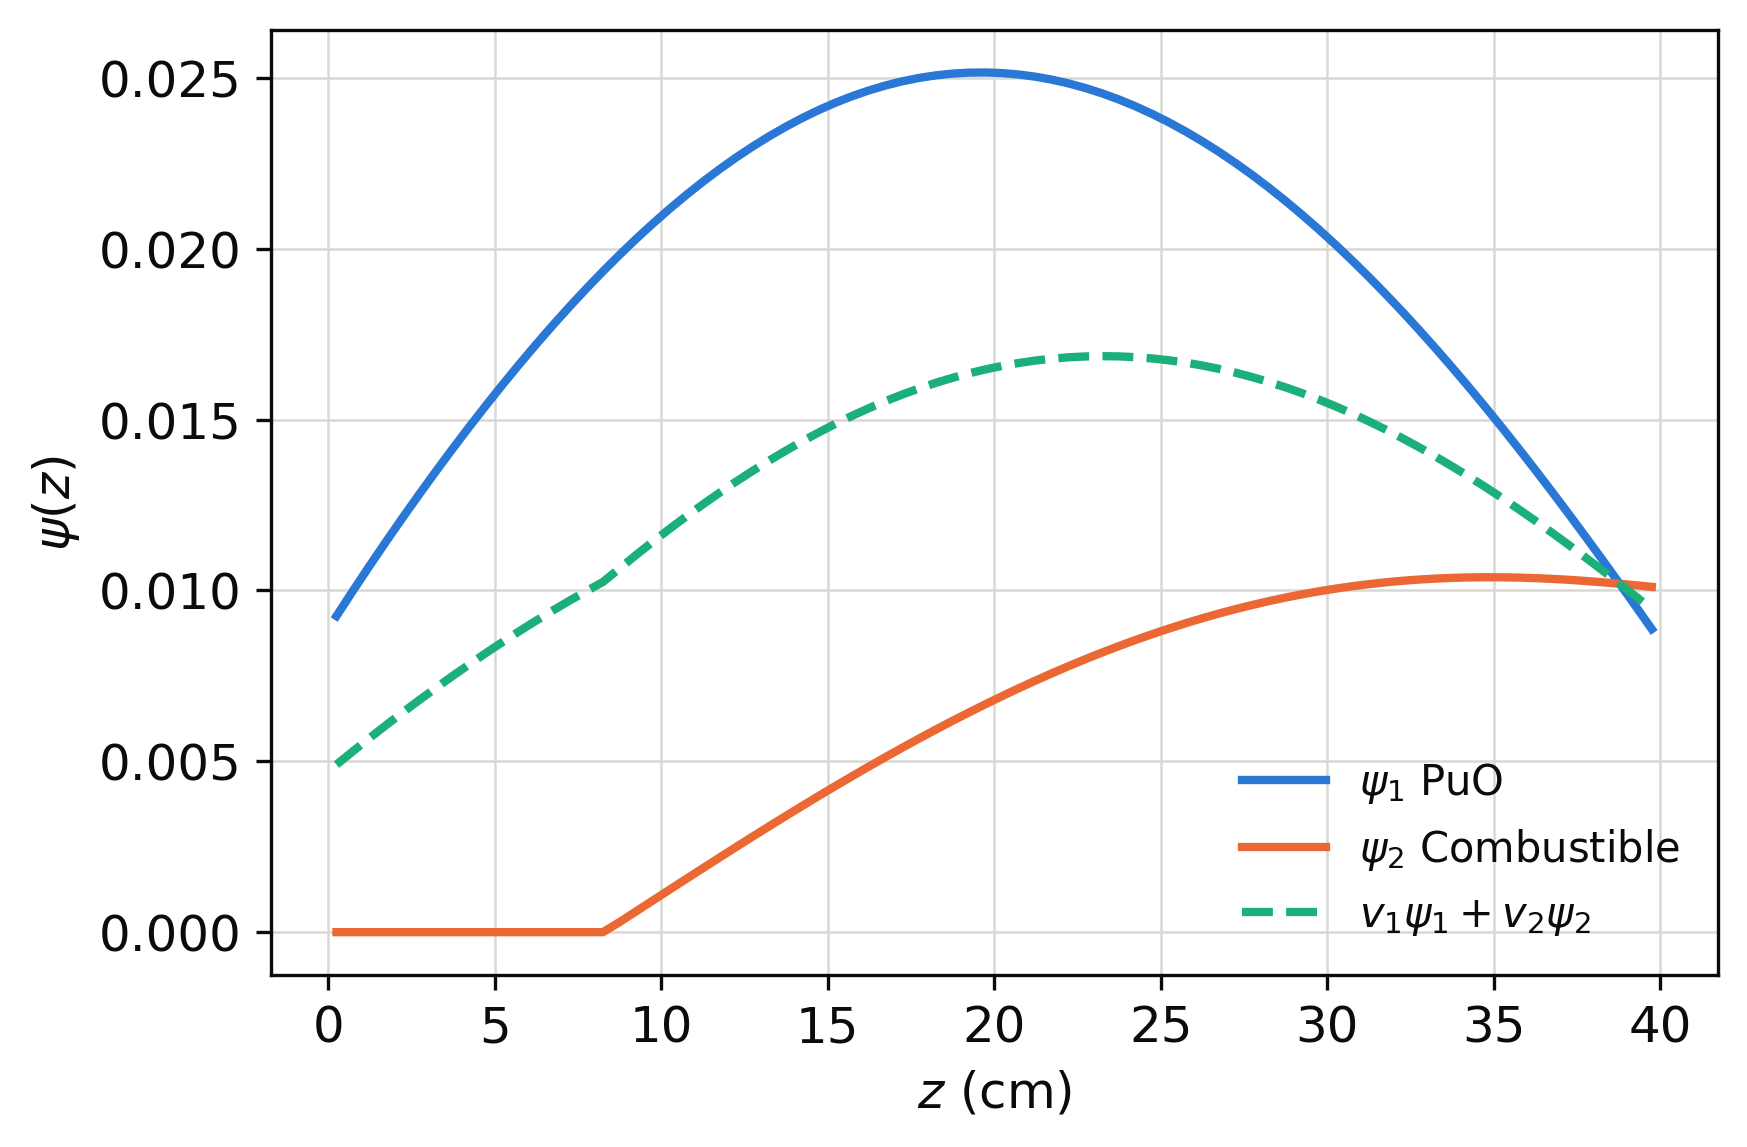
\includegraphics[width=0.7\textwidth]{fig_flux_spatial.png}
%     \caption{Flux shape function $\psi(z)$ at $t=300\,\mathrm{s}$ for
%     each phase and their volume-weighted combination. The visible
%     skew away from a symmetric (cosine-like) profile is not
%     numerical error: it is the direct consequence of the odd-order
%     drift terms in Eq.~89, which enter with a fixed spatial sign
%     because the correlation function $R(z) = e^{-\mu z}$ (Eq.~83) is
%     one-sided in $z$. The two phases skew in opposite directions
%     (PuO toward $z=0$, combustible toward $z=H$) since their
%     self-drift coefficients $\mu(1-v_i)$ differ; the combination does
%     not cancel this since $v_1 \neq v_2$ and the two flux magnitudes
%     differ substantially.}
%     \label{fig:flux_spatial}
% \end{figure}

% \begin{figure}[h]
%     \centering
%     
\includegraphics[width=0.7\textwidth]{fig_fuel_fraction.png}
%     \caption{Fuel mass fraction $\omega(z)$ at $t=300\,\mathrm{s}$.
%     PuO undergoes no pyrolysis by construction ($k_1=0$ in
%     Eq.~96). The combustible phase shows near-complete depletion
%     within the heated region close to $z=0$, falling off sharply
%     beyond roughly $5\,\mathrm{cm}$ where the temperature has not
%     risen enough to drive appreciable Arrhenius decomposition on the
%     simulated timescale.}
%     \label{fig:fuel_fraction}
% \end{figure}




% % \section{A two phase cylindrical system}
% % We now hone in on a particular two component system (PuO and another averaged combustible mix of metals and plastics). The geometry is cylindrical, with aziumthal symmetry. So we will use
% % \begin{align}
% %     \nabla f &= \frac{\partial f}{\partial r} \mathbf{\hat{r}}+\frac{\partial f}{\partial z} \mathbf{\hat{z}} \\
% %     \nabla \cdot \mathbf{A} &=\frac{1}{r}\frac{\partial}{\partial r}(rA_r)+\frac{\partial A_z}{\partial z} \\
% %     \nabla ^2 f&=\frac{1}{r} \frac{\partial}{\partial r}\left(r\frac{\partial f}{\partial r}\right) +\frac{\partial ^2 f}{\partial z^2}.
% % \end{align}
% % And for the correlation function 
% % \begin{equation}
% %     R(\mathbf{r})=e^{-\mu_r r-\mu_z z}
% % \end{equation}
% % so that 
% % \begin{equation}
% %     \nabla  R(\mathbf{r}) |_{\mathbf{r}=\mathbf{0}}= -\mu_r \hat{r}-\mu_z \hat{z}.
% % \end{equation}
% % It should suffice in our case to have $\mu_r =\mu _z$.


% \subsection{The Solve}
% We will solve our system of equations as follows: \\

% \textbf{Static flux solve}. At the start of each timestep, we must solve the eigenvalue problem 
% \begin{equation}
%     (L_i+A_i) \psi_i^g+\frac{1}{k} \chi_{eff}^g F_i \psi_i ^g=0
% \end{equation}
% with 
% \begin{align}
%     A_i \psi_i ^g &=-\Sigma_{a,i}^g \psi_i ^g +\sum_{g'=1}^G \Sigma_{s,i}^{g'\rightarrow g}\psi_i ^g \\
%     F_i \psi_i &= \sum_{g'=1}^G\nu_{g'}\Sigma_{f,i}^{g'} \psi_i ^{g'} \\
%     \chi_{eff}^{g}&=(1-\beta)\chi_p^g +\sum_j\beta_j \chi_{d,j}^g
% \end{align}
% and 
% \begin{multline}
%     L \psi_i = 
% \end{multline}




% The working neutronics equations are 
% \begin{equation}
%     \mathbf{Q}_i=-D_i \nabla \phi_i +D_i  \sum_j v_j (\phi_i - \phi_j)\nabla R(\mathbf{r})|_{\mathbf{r}=0}.
% \end{equation}
% So we have 
% \begin{equation}
%     \nabla \cdot \mathbf{Q}_i=
% \end{equation}




% Substituting in and rearranging we get 
% \begin{align}
%     \frac{1}{\upsilon} \frac{\dot{P}}{P}\psi_i &=L_i \psi_i +A_i\psi_i +(1-\beta)\chi_p F_i\psi_i+\sum_{j=1}^I\lambda_j \chi_{d,j}\hat{C}_{ji} \\
%     \frac{\dot{P}}{P}\hat{C}_{ji}&=\beta_j F_i\psi_i-\lambda_j \hat{C}_{ji}.
% \end{align}
% We will now take the inner product with the adjoint flux $\psi^\dagger_j (\mathbf{r})$ over space and energy groups in order to extract scalar solutions. We must also sum over all phases:
% \begin{align}
%     \dot{P}\sum_i \left<\psi_i^\dagger , \psi _i \right> 
% \end{align}
    
\end{document}